\chapter{Discussion} \label{sec:discussion}

In this section, we analyse the implications of the design and experimentation on the subject-driven augmentation pipeline we developed. The extensive experiments conducted provide evidence that subject-driven augmentation holds its own against other widely used techniques in the field of data augmentation. In particular, our generative approach is especially useful when the number of images available for training a computer vision model is limited. In particular, in our findings, we find an improvement of up to 19.11\% over the accuracy on the Oxford-IIIT Pet dataset when using 5\% of the original training set. Moreover, we show that it is possible to improve this result by adding conditional control. Latterly, considering this case, we obtain improvements of up to 23.47\%. 

Nevertheless, we do not stop there, and we extend our investigation to show that competitive computer vision models can be trained exclusively using synthetic images. However, it is important to acknowledge that a disparity still exists between models trained with synthetic images and those trained with real ones. Finally, we prove that subject-driven augmentation is extensible to other tasks, such as segmentation and generalisable to other datasets, such as Food-101.

Let us consider these results alongside the research question, which asked, to what extent can images generated by text-to-image systems improve the performance of computer vision models? In doing so, we can draw the following implications.

\begin{itemize}
    \item Subject-driven augmentation techniques are a valid and competitive approach to data augmentation.
    \item Subject-driven augmentation techniques are especially relevant in datasets where data is scarce or expensive to obtain.
    \item There is still a relevant gap between synthetic and real images.
\end{itemize}

The question then arises, how do these implications affect or contribute to the field of computer vision? 

One of the first effects that stands out in importance is that \textbf{the cost of creating large, quality datasets is reduced}. The scientific community has paid more attention to improving architectures than improving and augmenting datasets \cite{ghiasi2021simple}. This is because it is extremely expensive to have large datasets with which to train deep learning architectures \cite{yang2022image}. Therefore, generative augmentation approaches allow \textit{few-shot} learning \cite{wang2020generalizing}. They allow a model to be trained to generalise and make accurate predictions with only a limited number of labelled examples for each class. For example, in the developed pipeline, with only 5 real images per class, we can customise a text-to-image model to generate as many images as desired from a category. Therefore, the capabilities of the models are greatly expanded when reduced information is available. Furthermore, the cost of creating datasets is reduced because there is no need for costly and time-consuming data annotation.

Nevertheless, there is no strict requirement to confine analyses solely to finite datasets, as it is conceivable, at a conceptual level, to contemplate an approach wherein the model encounters each training image only once \cite{parisi2019continual}. In this way, with a sufficiently expressive text-to-image model, sets of images could be provided that would, in practice, be unlimited \cite{sariyildiz2023fake}. However, despite the logical coherence of this concept, its actual implementation is unfeasible due to the imperfect expressiveness of current models.

Another possibility that we study that derives from the idea of \textit{few-shot} learning is \textit{zero-shot} learning, i.e. no real-world training data is available. At a conceptual level, what is being done is a transfer of information from the text-to-image model to a model specialised in another task. It is true, however, that this concept is also present in the \textit{few-shot} learning scheme. Nevertheless, the fact that there is no real data implies that, in practical terms, all the information with which the task is learned comes from the text-to-image model \footnote{Assuming that there is no pre-trained model}. Our data imply that it is possible to obtain usable results with \textit{zero-shot} learning. However, we found that \textbf{there is still a significant gap between synthetic and real images}. Thus, it is not possible to obtain the performance of trained models with a sufficient amount of real images regardless of the number of synthetic images used.

The present study adds to a large body of literature investigating the possibilities of synthetic imaging. As this area has recently been revolutionised by the increasing capabilities of text-to-image models \cite{ho2020denoising, dhariwal2021diffusion}, there is much interest from the scientific community. Other relevant works in the area are the following. In \cite{sariyildiz2023fake}, the authors explore Stable Diffusion's ability to create ImageNet clones to train classification models from scratch using only class names. In \cite{azizi2023synthetic}, they augment the ImageNet dataset with synthetic images achieving state-of-the-art results. In \cite{trabucco2023effective}, the researchers increase the diversity of a dataset with image-to-image transformations performed with a text-to-image model. Finally, in \cite{he2022synthetic}, they explore how synthetic images can help in \textit{zero-shot} and \textit{few-shot} tasks. All these works draw conclusions that align with those proposed in the present research and, thus, support our conclusions.

Despite the relative success in addressing the research question, the present study has some limitations. Among the most important is the instability in obtaining consistently good images. As shown in section \ref{sec: results}, many of the images we have generated are of excellent quality and may even confuse some people. However, we have observed that they also generate bad images in a way that we cannot control. Figure \ref{fig:low-quality} shows some of these particularly bad images. 

\begin{figure}
    \centering
    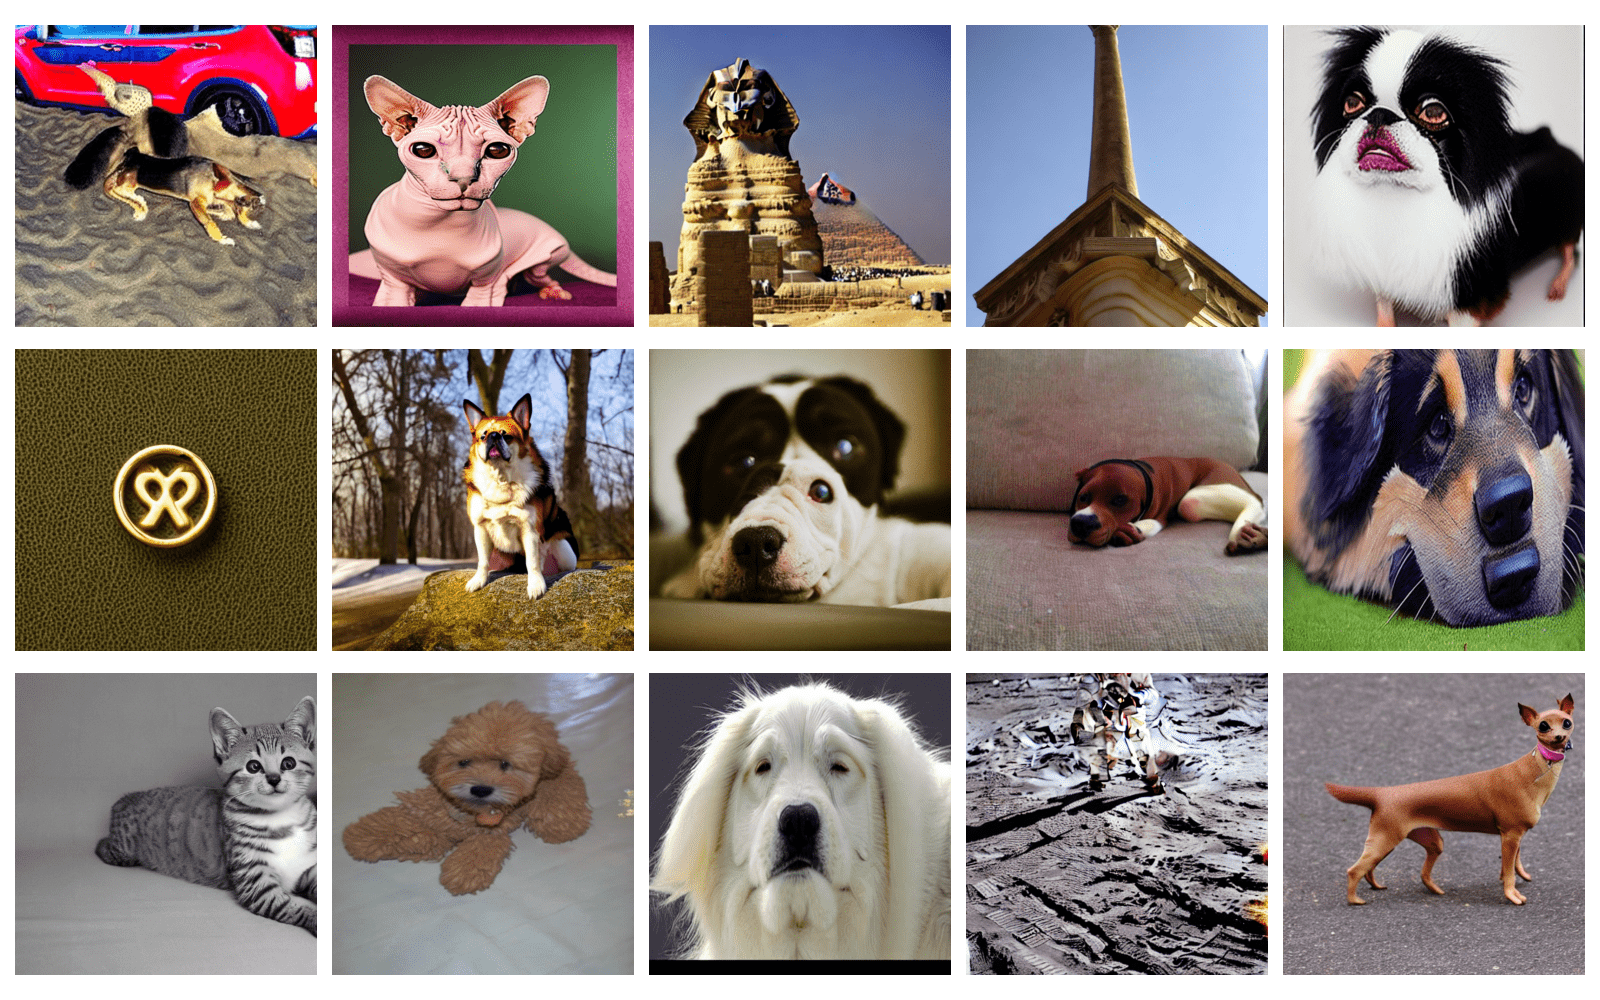
\includegraphics[width=1\textwidth]{Pictures/low-quality-img.png} 
    \caption{\textbf{Synthetic images exhibiting anomalies}. Artefacts, deformations, and subject absence are prevalent among the frequently encountered anomalies.}
    \label{fig:low-quality}
\end{figure}

This type of images may explain some of the instabilities found in some graphs, such as \ref{fig:exp4} or \ref{fig:exp8}, where the accuracy shows points with strange behaviour. One of the solutions that can be applied is to perform multiple runs of the image generation to take the average. While it is true that we have tried to run the runs a minimum of 2 times, this is insufficient and still allows for instabilities caused by stochastic processes. The reason why we have not run the tests more times is that they are very demanding in terms of time and computational resources. Therefore, this fact presents a weakness of our study that can be improved with more time or more polished and optimised algorithms.

Finally, another particularly relevant problem from a social perspective is that of bias. Although in this work, we have dealt with domains where this problem is not particularly worrying (animals and food), we must warn of the dangers that we observe in this area. \textbf{Large text-to-image models inherit the biases present in the data used to train them}. Most of this data comes from the internet and clearly presents significant problems. For example, DALL-E 2 makes assumptions about race or gender with specific tasks or jobs as detailed by its creators in \cite{DALLR}. Therefore, stereotypes and biases are carried over and amplified by using the synthetic images generated by the text-to-image models. However, there are techniques to limit these problems. For example, the creators of Textual inversion present how their technique can be used to reduce bias \cite{gal2022image}. Their approach involves making the model learn new pseudo-words for familiar concepts such as CEO or nurse. Image \ref{fig:bias-textual} shows the results they achieve by applying their technique to bias and stereotype reduction.

\begin{figure}
    \centering
    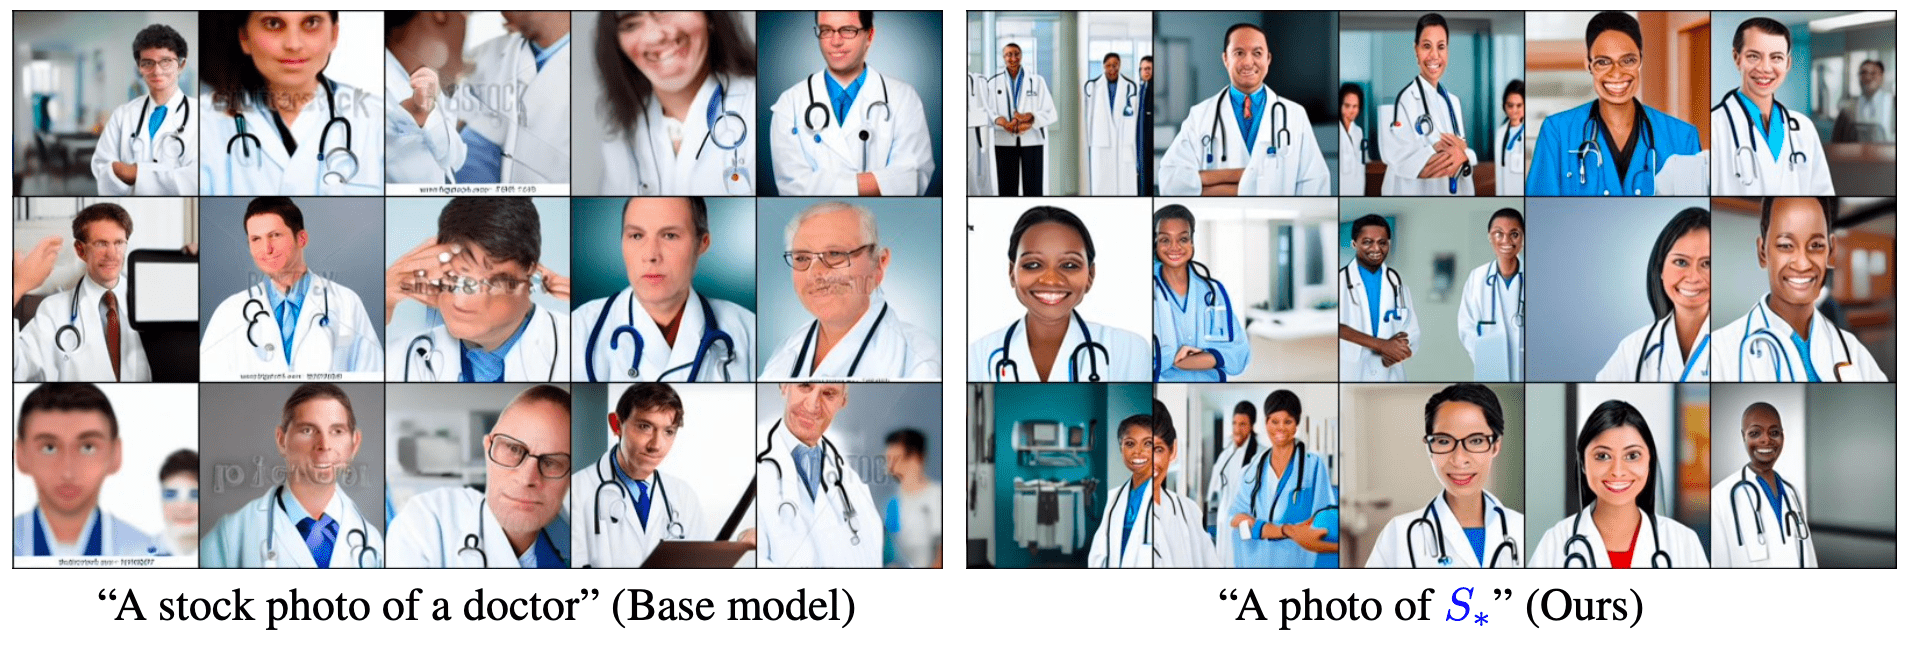
\includegraphics[width=1\textwidth]{Pictures/bias-text.png} 
    \caption{\textbf{Bias reduction using Textual inversion} \cite{gal2022image}. Samples obtained from the pretrained biased embeddings (left) and the debiased embeddings (right). The methodology facilitates bias reduction by acquiring novel pseudo-words representing established concepts. These pseudo-words can be fine-tuned using datasets thoughtfully curated for bias reduction.}
    \label{fig:bias-textual}
\end{figure}

In summary, in this paper, we demonstrate that images generated by text-to-image models can improve the performance of computer vision models and draw relevant implications in the field of deep learning. \textbf{Subject-driven augmentation techniques are especially relevant in datasets where data is scarce or expensive} to obtain (\textit{few-shot} learning). On the other hand, there is still a \textbf{relevant gap between synthetic and real images} that prevents competitive results in \textit{zero-shot} learning.
